\chapter[ADNEX model systematic review and meta-analysis]{The ADNEX risk prediction model for ovarian cancer diagnosis: A systematic review and meta-analysis of external
validation studies}
% Only include if the thesis is written as a collection of papers
%_________________________
\includegraphics*[width=0.8\linewidth]{logos/BMJ_Medicine.png}
\label{sec:chp_ADNEXSR}

\glsunset{ADNEX}
\glsunset{AUC}
\glsunset{CHARMS}
\glsunset{CI}
\glsunset{CrI}
\glsunset{ESGE}
\glsunset{ESGO}
\glsunset{GRADE}
\glsunset{IOTA}
\glsunset{ISUOG}
\glsunset{JAGS}
\glsunset{NB}
\glsunset{OSF}
\glsunset{PI}
\glsunset{PRISMA}
\glsunset{PROBAST}
\glsunset{QUADAS}
\glsunset{ROC}
\glsunset{RU}
\glsunset{TRIPOD}


published as: 
\begin{quote}
 \textbf{Barreñada L}, Ledger A, Dhiman P et al. ADNEX
risk prediction model for diagnosis of ovarian cancer: systematic review and
meta-analysis of external validation studies. \textit{BMJ Medicine}. 2024;3:e000817. \url{https://doi.org/10.1136/bmjmed-2023-000817}

\end{quote}
\begin{quote}
 \textbf{Supplementary material and code} available in the online version and at \url{https://osf.io/jtsvd/}.
\end{quote}
\vspace{-0.5em}
\noindent\scriptsize\textit{Submitted: 17/11/2023 \quad Published: 17/02/2024 \quad (123 days) \quad APC: 3580 \pounds}
\normalsize\vspace{-0.5 em}
%_________________________
\section*{Summary}
We performed a systematic review and meta-analysis of 47 external validation studies of the ADNEX model, covering more than 17,000 tumours. Most validations (91\%) were judged to be at high risk of bias, primarily because studies excluded cases with missing data without explanation, enrolled small samples, or did not assess calibration. Overall methodological reporting was poor according to TRIPOD checklist. Despite these limitations, ADNEX showed good discrimination between benign and malignant tumours across countries and clinical settings, irrespective of whether CA125 was included. However, calibration was infrequently reported, which did not allow for a comprehensive assessment of predicted risks. Systematic review registration PROSPERO CRD42022373182.

\newpage

\section{Introduction}

The optimal management of patients with an ovarian mass depends on the histology
of the mass. Patients with a benign mass can be managed non-surgically with
clinical and ultrasound follow-up or using conservative surgical techniques 
 \cite{carleyLaparoscopyLaparotomyManagement2002,
froymanRiskComplicationsPatients2019}.
Malignant tumours benefit from management in specialised oncology centres, but invasive tumours may require different surgical approaches
 \cite{wooCentralisationServicesGynaecological2012,
timmermanESGOISUOGIOTA2021}.
To optimise patient triage without operating on all masses, diagnostic models
can be used to estimate the likelihood of malignancy and so be used to plan
treatment for patients.

Given the potential advantages of accurately predicting risk of malignancy, the
International Ovarian Tumour Analysis (\gls{IOTA}) group developed the Assessment of
Different NEoplasias in the adneXa (\gls{ADNEX}) risk prediction model, using three
clinical and six ultrasound predictor variables
 \cite{vancalsterEvaluatingRiskOvarian2014}. The clinical variables are age,
serum CA-125 level, and type of centre (oncology centre vs other). An oncology
centre is defined as a tertiary referral centre with a specific gynaecology
oncology unit. The ultrasound variables are the maximal diameter of the lesion,
proportion of solid tissue (defined as the largest diameter of the largest solid
component divided by the largest diameter of the lesion), number of papillary
projections, presence of more than 10 cyst locules, presence of acoustic
shadows, and ascites. \gls{ADNEX} is a multinomial logistic regression model that estimates the risk of five
tumour types: benign, borderline, stage I primary invasive, stage II-IV primary
invasive, and secondary metastatic.

The total risk of malignancy calculated by
\gls{ADNEX} is the sum of the risks for each malignant subtype. \gls{ADNEX} has two
versions: one with and one without CA125 as a predictor (the \gls{ADNEX} formulas are
provided in Supplementary material S1)
 \cite{vancalsterEvaluatingRiskOvarian2014}. When we refer to \enquote{the \gls{ADNEX} model}
or \enquote{\gls{ADNEX}}, we refer to both versions of the model. The model was developed on
data from 5909 patients with an adnexal mass that subsequently underwent surgery
and that were recruited at 24 centres across 10 countries (Belgium, Italy, Czech
Republic, Poland, Sweden, China, France, Spain, UK and Canada). Although
developed on data from patients that underwent surgery, the performance of \gls{ADNEX}
has been evaluated also on cohorts that included non-surgically managed patients
 \cite{vancalsterValidationModelsDiagnose2020,
hackExternalValidationORADS2022,
jeongValidationIOTAADNEXModel2020,
quarantaSurgeryBenignOvarian2020}.

\gls{ADNEX} is included in national guidelines, e.g. in Belgium, The Netherlands and
Sweden
 \cite{RegionalaCancercentrumSamverkan2023,
ignaceEierstokkankerDiagnoseBehandeling2016,geominipZonMwProjACCEPTAccuracy2021}.
It is recommended by scientific societies, such as International Society of
Ultrasound in Obstetrics and Gynecology (\gls{ISUOG}), European Society of
Gynaecological Oncology (\gls{ESGO}), European Society for Gynaecological Endoscopy
(\gls{ESGE}), and the American College of Radiology
 \cite{timmermanESGOISUOGIOTA2021,
andreottiORADSUSRisk2020}. In addition,
manufacturers of ultrasound machines have begun to incorporate \gls{ADNEX} directly
into their machines.

Several external validation studies of \gls{ADNEX} have been carried out. To date,
five published systematic reviews and meta-analyses of \gls{ADNEX} have summarised
between 3 and 22 external validation studies
 \cite{cuiDiagnosticAccuraciesUltrasound2022,
davenportMenopausalStatusUltrasound2022,
huangDiagnosticAccuracyADNEX2021,
westwoodRiskScoresGuide2018,
yueValueAssessmentDifferent2022}.
All of the systematic reviews evaluated \gls{ADNEX} only as a diagnostic test, reporting a
summary sensitivity and specificity at a threshold for the estimated risk of
malignancy of 10\% or 15\%
 \cite{cuiDiagnosticAccuraciesUltrasound2022,
davenportMenopausalStatusUltrasound2022,
huangDiagnosticAccuracyADNEX2021,
westwoodRiskScoresGuide2018,
yueValueAssessmentDifferent2022}.
The ADNEX model not only classifies masses as benign or malignant, however, it can also be used as a risk prediction model, providing probability estimates for five different tumour types at the individual patient level. Hence focusing only on its performance in classifying tumours, risks losing useful information \cite{onbehalfofthetopicgroupevaluatingdiagnostictestsandpredictionmodelsofthestratosinitiativeThreeMythsRisk2019}. When validating ADNEX as a diagnostic test at a 10\% threshold, the performance metrics (ie, sensitivity and specificity) do not take into account the individual risks predicted but the same weight is given to a misclassified patient with an 11\% risk as with a 99\% risk. This approach means that these meta-analyses have not fully validated the diagnostic performance of ADNEX; for example, pooling discrimination performance (area under the receiver operating characteristic curve, \gls{AUC}) allows determination of the ability of the model to differentiate between patients with and without the outcome across different thresholds. Guidelines on how to evaluate the quality and risk of bias of external validation studies of risk prediction models have been produced.
 \cite{debrayGuideSystematicReview2017,
wolffPROBASTToolAssess2019,
snellTransparentReportingMultivariable2023}.These guidelines should be used in meta-analyses of validation studies. Hence the objectives of this study were to perform a systematic review of studies that externally validated ADNEX, to describe reporting completeness and risk of bias of the validation studies, and to conduct meta-analyses of measures of performance of the model.

\section{Methods}

\subsection{Protocol registration}
We report this study according to the \gls{PRISMA} (Preferred Reporting Items for
Systematic reviews and Meta-Analysis, online supplemental file 2) and \gls{TRIPOD}-SRMA (Transparent Reporting of
multivariable prediction models for Individual Prognosis Or Diagnosis: checklist
for Systematic Reviews and Meta-Analyses, supplemental file 3) checklists
 \cite{snellTransparentReportingMultivariable2023,
pagePRISMA2020Statement2021}.

\subsection{Eligibility criteria}
Any study that carried out an external validation to evaluate the performance of the ADNEX model, based on any study design and any study population, was eligible for inclusion in the systematic review. Exclusion criteria were studies that did not evaluate the performance of the ADNEX model; studies that only evaluated the predictive performance of updated versions of ADNEX; studies where only an abstract was available, or the full text could not be obtained; and case studies presenting the performance of ADNEX for individual patients (this criterion was not prespecified in the protocol but was added post hoc on review of the search results). Updating can refer to recalibration, refitting, or extension with additional predictors
 \cite{steyerbergClinicalPredictionModels2009}. Studies that conducted comparisons of ADNEX with other models, reporting performance metrics, were eligible for inclusion.

\subsection{Information sources and search strategy}
We created a search string and overall search strategy with the help of
biomedical reference librarians of the KU Leuven Libraries. We searched the
electronic databases Medline (via PubMed), EMBASE, Web of Science, and Scopus
for published articles, and EuropePMC for preprints. The search dates were from
the publication of the first \gls{ADNEX} paper (15/10/2014) until 15/05/2023 (date the
final search was run). We also screened all articles citing the original \gls{ADNEX}
paper \cite{vancalsterEvaluatingRiskOvarian2014}. The reference lists of
relevant review and opinion articles retrieved by the search strings were
checked for other potentially eligible articles. Forward and backward
snowballing (forward/back cross-reference checking) of the included articles was
performed to identify additional publications \cite{wohlinGuidelinesSnowballingSystematic2014}. Language was not restricted, but for papers in languages other than English, Spanish, Dutch, French, or Swedish, we used an automatic translation tool (\url{https://deepl.com}) to decide whether to include a paper and to extract information. Online supplemental material S2 shows the full search strategy.

\subsection{Study selection}
The studies we identified in our search were imported into Zotero reference manager, where they were automatically deduplicated. The deduplicated records were then imported into the Rayyan web application for manual deduplication (by LB) and subsequent screening of the title and abstract by two independent authors. Disagreements were resolved by discussion between the two authors (LB and AL) \cite{ouzzaniRayyanWebMobile2016}.

Three of the authors (BVC, LV, and DT) were members of the IOTA group that developed ADNEX, so we divided the studies into those that were linked or not linked to IOTA. A study was linked to IOTA if it was coauthored by a member of the IOTA steering committee (online supplemental material S3). IOTA linked papers, as well as a few others with a potential conflict of interest (ie, including authors that are or were IOTA collaborators), were independently assessed by two of the authors (PD and GSC, medical statisticians with expertise in prediction modelling and unrelated to IOTA). All other studies were independently assessed (by LB and AL). Disagreements were resolved by discussion between reviewers, and for the non-IOTA papers, by discussion with authors BVC, LV, and JYV.

\subsection{Data extraction and data items}
Data were extracted and entered into a standardised data extraction form in Microsoft Excel. Data extraction focused on the general and design characteristics of the studies, target population, reference standard, sample size, performance results, reporting quality, methodological quality, and risk of bias (online supplemental table S1). The extraction form was adapted from the CHARMS (CHecklist for critical Appraisal and data extraction for systematic Reviews of prediction Modelling Studies) and TRIPOD (Transparent Reporting of a multivariable prediction model for Individual Prognosis Or Diagnosis) tools, and PROBAST (Prediction model Risk Of Bias Assessment Tool) \cite{wolffPROBASTToolAssess2019,
moonsCriticalAppraisalData2014,
collinsTransparentReportingMultivariable2015}.

To describe the performance of the model, we extracted information on any reported measure related to discrimination, calibration, diagnostic accuracy, or clinical utility. The reference standard could be binary (eg, benign v malignant) or multinomial (eg, the five tumour types predicted by ADNEX). Performance data were extracted for all reported validations (ie, for ADNEX with and without CA125), subgroup analyses, sensitivity analyses, and for multicentre studies, results specific to each centre. For each study, we assessed the reporting of all TRIPOD items that were applicable to the external validation studies (online supplemental table S2). We also checked PROBAST’s signalling questions and evaluated risk of bias for each subdomain (participants, predictors, outcome, and analysis) and overall. We included our rationale for classification of the risk of bias.

We contacted study authors to obtain further information or results when centre specific results were not reported in multicentre studies, type of centre was not explicitly reported (if no response, the clinical coauthors, JYV, DT, and LV, classified the centre), overall performance was reported but not performance by menopausal status, or performance was not reported for patients who underwent surgery separately in studies that included patients who were managed surgically and non-surgically. Online supplemental table S1 and Open Science Framework repository (extraction sheet, \url{https://osf.io/jtsvd/}) have details on all extracted items \cite{barrenadaADNEXRiskModel2025}.

\subsection{Statistical analysis and quantitative data synthesis}
Data were summarised with descriptive statistics and data visualisations. Meta-analysis of performance, based on specific results for each centre in multicentre studies, where possible, was conducted with the random effects meta-analysis method. Meta-analysis was done separately for ADNEX with and without CA125. We used 95\% confidence intervals for the summary performance and assessed heterogeneity with $\tau^2$ and 95\% prediction intervals. Online supplemental material S4-6 have details on the statistical methodology, including meta-analysis methods, explanations of net benefit and relative utility, and assessment of publication bias.

Meta-analysis of the \gls{AUC} for benign versus malignant tumours was done on the
logit scale. Meta-analysis for sensitivity and specificity was also performed on
the logit scale using random effects meta-analysis
 \cite{rileyBivariateRandomeffectsMetaanalysis2007}. Because the meta-analysis was conducted only for the 10\% threshold for the risk of malignancy, we did not need the 95\% confidence ellipse in receiver operating characteristic curve space, so we did not use the bivariate random effects model as specified in the protocol. The 10\% threshold was most commonly used in the articles included in our systematic review, and is a commonly recommended threshold \cite{timmermanESGOISUOGIOTA2021}. Meta-analysis of Net
Benefit (\gls{NB}) \cite{vickersDecisionCurveAnalysis2006} and Relative Utility (\gls{RU})
 \cite{bakerPuttingRiskPrediction2009} at the 10\% risk of malignancy threshold
was performed  with bayesian trivariate random effects meta-analyses of sensitivity, specificity, and prevalence of malignancy \cite{wynantsRandomeffectsMetaanalysisClinical2018}. For bayesian methods, 95\% credible intervals are reported instead of 95\% confidence intervals. With the bayesian approach, the probability that the model is useful in a new centre can be estimated (ie, the probability that relative utility is >0). To deal with multinomial discrimination performance, we conducted a meta-analysis of AUC values between pairs of tumour outcomes (pairwise AUC values) on a logit scale. We only included studies that used the conditional risk method to calculate pairwise AUC values \cite{vancalsterAssessingDiscriminativeAbility2012}. 

Subgroups were defined based on geographical location, type of centre, and menopausal status. Sensitivity analyses were based on judgment of the risk of bias and on whether the study was linked to IOTA. As prespecified in the protocol, we only conducted a meta-analysis of performance if at least three estimates in a specific analysis could be retrieved from the included studies. To assess the association between prevalence of malignancy and AUC, and sensitivity and specificity at the 10\% risk of malignancy threshold, we used meta-regression \cite{thompsonHowShouldMetaregression2002}.

Reporting bias and small study effects were visually explored using funnel plots
adapted for the \gls{AUC}. The body of evidence was assessed with an adapted version
of \gls{GRADE} \cite{guyattGRADEEmergingConsensus2008}. All analyses were performed in
R version 4.2.2 using package \texttt{metamisc} for the \gls{AUC}, \texttt{meta} and \texttt{mada} for
sensitivity and specificity, and \texttt{rjags} for \gls{NB} and \gls{RU}
 \cite{debrayFrameworkMetaanalysisPrediction2019,
schwarzerMetaAnalysis2015,
doeblerMetaanalysisDiagnosticAccuracy2025,
plummerRjagsBayesianGraphical2023}.
Bayesian methods were computed using \gls{JAGS} version 4.3.1
 \cite{plummerRjagsBayesianGraphical2023}.

\subsection{Patient and public involvement}
Patients and the public were not involved in the design, or conduct, or reporting, or dissemination plans of this research. Preliminary results of the research were presented at the ISUOG World Congress in Seoul (October 2023). As this study was a systematic review, there was no collection of patients' data, and we use only the information publicly available in the published papers.

 \begin{table}[h!]
\small
\centering
\caption{Characteristics of the 47 included studies.}
\label{tab:1}
\begin{tabularx}{\linewidth}{l c >{\raggedright\arraybackslash}X}
\toprule
\textbf{Study characteristic} & \textbf{No (\%)} & \textbf{Comments} \\ 
\midrule
\textbf{Unit of analysis} & & \\
\quad Patient & 42 (89) & 1 tumour per patient \\
\quad Tumour & 5 (11) & >1 tumour per patient possible \\
\addlinespace
\textbf{Region} & & \\
\quad Asia & 24 (51) & Common countries: China (12), South Korea (3) \\
\quad Europe & 18 (38) & Common countries: Poland (7), Italy (4), Spain (4), UK (3), Sweden (3) \\
\quad South America & 3 (6) & \\
\quad North America & 2 (4) & \\
\addlinespace
\textbf{Number of centres} & & \\
\quad 1 & 37 (79) & \\
\quad 2-5 & 7 (15) & \\
\quad >5 & 3 (6) & Range: 8-17 \\
\addlinespace
\textbf{Type of centre} & & \\
\quad Oncology centre(s) & 35 (74) & \\
\quad Non-oncology centre(s) & 2 (4) & \\
\quad Both types of centres & 4 (9) & \\
\quad Unclear & 6 (13) & \\
\addlinespace
\textbf{ADNEX version} & & \\
\quad \gls{ADNEX} with CA125 & 37 (79) & 21 only used \gls{ADNEX} with CA125, 16 used both \\
\quad \gls{ADNEX} without CA125 & 19 (40) & 3 only used \gls{ADNEX} without CA125, 16 used both \\
\quad Mixed & 3 (6) & \gls{ADNEX} with CA125 used if CA125 was available \\
\quad  Unclear & 4 (9) & \\
\addlinespace
\textbf{Selection based on histology} & & \\
\quad No & 39 (83) & \\
\quad Yes & 8 (17) & e.g., borderlines excluded, only invasive tumours \\
\addlinespace
\textbf{Focus only on clinical subgroup} & & \\
\quad No & 42 (89) & \\
\quad Yes & 5 (11) & e.g., only pregnant patients \\
\addlinespace
\textbf{Target population} & & \\
\quad Patient who underwent surgery & 43 (91) & \\
\quad  Patients who did or did not undergo surgery & 4 (9) & \\
\bottomrule
\end{tabularx}
\end{table}


\section{Results}

\begin{figure}
\centering
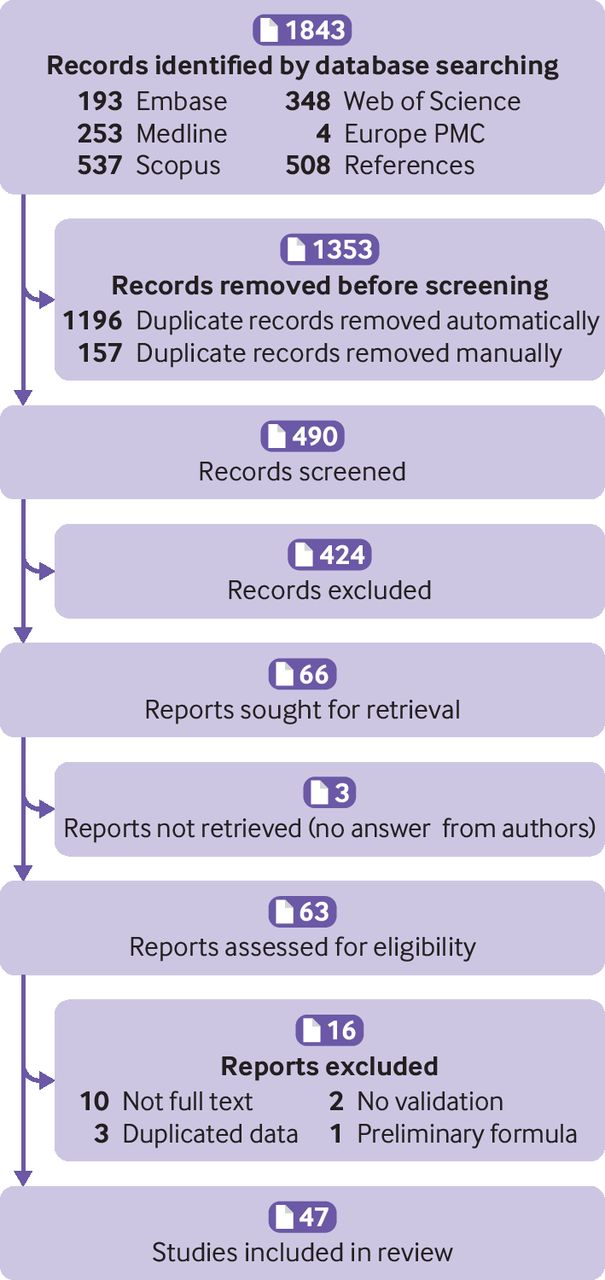
\includegraphics[scale=1]{figures/ADNEXSR/F1.jpg}
\caption[PRISMA flowchart]{PRISMA (Preferred Reporting Items for Systematic Reviews and Meta-Analyses) flowchart of study inclusions and exclusions.}
\label{fig:1:1}
\end{figure}



We identified 1843 records and screened 490 duplicates were removed. Forty-seven
studies met our inclusion criteria and were included in this systematic review
(Figure \ref{fig:1:1}, Table S3)
 \cite{vancalsterValidationModelsDiagnose2020,
hackExternalValidationORADS2022,
jeongValidationIOTAADNEXModel2020,
quarantaSurgeryBenignOvarian2020,
araujoPerformanceIOTAADNEX2017,
behnamfarComparisonUltrasoundTumor2022,
budianaSkorAssessmentDifferent2022,
butureanuOvarianMassesapplicableIota2021,
chenComparisonORADSADNEX2022,
chenPerformanceIOTAADNEX2019,
czekierdowskiSonographicAssessmentComplex2021,
czekierdowskiPerformanceIOTASimple2023,
diazOvarianTumorsRisk2017a,
epsteinSubjectiveUltrasoundAssessment2016,
esquivelvillabonaTwoStepStrategyOptimizing2022,
gaurilcikasPerformanceIOTAADNEX2020,
heEstimatingRiskMalignancy2021,
hiettPerformanceIOTASimple2022,
huComparisonUltrasoundbasedADNEX2023,
jiangOvarianSexCord2021,
jianhongComparisonPerformanceORADS2022,
joyeuxSurgeryPredictabilityMalignant2016,
laiComparisonORADSGIRADS2022,
lamhuongOptimalCutOffPoint2022,
leeUltrasonographicEvaluationOvarian2021,
liuADNEXModelbasedDiagnosis2021,
meysEstimatingRiskMalignancy2017,
namAssessmentDifferentNEoplasias2021,
nohuzReliabilityIOTAScore2019,
pelayoComparisonUltrasoundScores2023,
pengEvaluationDiagnosticValue2021,
poonyakanokPreoperativeEvaluationADNEX2021,
qianComparisonDiagnosticPerformances2021,
rashmiDiagnosticPerformanceUltrasoundBased2023,
sandalComparisionRiskMalignancy2018a,
sayasnehEvaluatingRiskOvarian2016,
stukanDevelopmentValidationModel2019,
stukanUltrasoundClinicalPreoperative2019,
szubertExternalValidationIOTA2016,
szubertPerformanceSelectedModels2020,
tavoraiteUltrasoundAssessmentAdnexal2021,
tugPreoperativeDiscriminatingPerformance2020,
velayoDiagnosticPerformancesUltrasoundBased2023,
vioraADNEXModelTriage2020,
wangEvaluatingRiskMalignancy2023,
yangPerformanceIOTAADNEX2022,
zhangExternalValidationAssessment2022}.
Three studies were excluded because the same data were used in another included study, and one study was excluded because a preliminary formula of ADNEX was used
 \cite{landolfoBenignDescriptorsADNEX2023,
poonyakanokProspectiveComparativeTrial2023,
froymanRiskComplicationsPatients2019,
wynantsClinicalUtilityRisk2017}.
The data of three studies that were linked to IOTA and three other studies with a potential conflict of interest were extracted by authors PD and GSC
 \cite{vancalsterValidationModelsDiagnose2020,
epsteinSubjectiveUltrasoundAssessment2016,
meysEstimatingRiskMalignancy2017,
sayasnehEvaluatingRiskOvarian2016,
stukanDevelopmentValidationModel2019,
szubertPerformanceSelectedModels2020}.




Table \ref{tab:1} summarises the key study characteristics and table S3 shows the specific details for each study. The unit of analysis was the patient in 42 (89\%) studies and the tumour in five (11\%) studies. When tumour was the unit of analysis, multiple tumours for the same patient could be included. The 47 studies reported on 17 007 tumours, with a median study sample size of 261 tumours (range 24-4905). Validations were conducted in 28 countries, with most studies conducted in Asia (51\%) and Europe (38\%). Online supplemental material S7 gives a list of reporting inconsistencies. All studies classified borderline tumours as malignant tumours.



\gls{ADNEX} with CA125 was validated in 37 (79\%) studies, and \gls{ADNEX} without CA125 in
19 (40\%) studies (16 studies evaluated both versions). For four (9\%) studies, the ADNEX version was unclear. In total, 63 validations of ADNEX were performed after distinguishing between the ADNEX versions used (online supplemental table S4). When reported results for subgroups (eg, by menopausal status or by centre in multicentre studies) were also included, the total number of validations reported for the 47 studies was 159. When also including reported results for subgroups (e.g., by
menopausal status, or by centre in multicentre studies), the total number of
validations reported across the 47 studies was 159.

Five (11\%) studies focused only on a specific clinical subgroup, such as pregnant patients or tumours, and the clinician's subjective assessment of the outcome was uncertain
 \cite{quarantaSurgeryBenignOvarian2020,
  czekierdowskiSonographicAssessmentComplex2021,
  leeUltrasonographicEvaluationOvarian2021,nohuzReliabilityIOTAScore2019,
  szubertPerformanceSelectedModels2020}.
Eight (17\%) studies selected patients based on histology (Table S3). Thirty six (77\%) studies did not focus on a specific clinical subgroup and did not select tumours based on histology. In these 36 studies that were eligible for the meta-analysis, median sample size was 284 tumours (range 50-4905), median number of malignant tumours was 68 (7-1041), and median prevalence of malignancy was 28\% (3–57\%). Fourteen of the 36 (39\%) studies had ≥100 benign and ≥100 malignant tumours.

\begin{table}[ht!]
\centering
\caption[Meta-analysis results of AUC]{Meta-analysis of the AUC to discriminate between benign and malignant tumours, including sensitivity and subgroup analyses.}
\label{tab:2}
\footnotesize
\begin{tabularx}{\textwidth}{>{\raggedright\arraybackslash}X >{\centering\arraybackslash}p{2cm} >{\centering\arraybackslash}p{3cm} c c}
\toprule
\textbf{Meta-analysis} & \textbf{No of studies (centres)} & \textbf{Summary estimate (95\% \gls{CI})} & \textbf{95\% PI} & \boldsymbol{\tau^2} \\
\midrule
\textbf{Main analysis} & & & & \\
Operated patients, with CA125 & 21~(43) & 0.93~(0.92-0.94) & 0.85~to~0.98 & 0.25 \\
Operated patients, without CA125 & 12~(31) & 0.93~(0.91-0.94) & 0.85~to~0.98 & 0.21 \\
\addlinespace
\textbf{Sensitivity analyses (operated patients)} & & & & \\
High or Unclear risk of bias studies, with CA125 & 19~(23) & 0.93~(0.91-0.95) & 0.84~to~0.99 & 0.33 \\
Low risk of bias studies, with CA125 & 2~(20) & 0.93~(0.91-0.94) & 0.87~to~0.97 & 0.12 \\
\gls{IOTA} studies, with CA125 & 4~(23) & 0.92~(0.91-0.94) & 0.88~to~0.97 & 0.09 \\
Non-\gls{IOTA} studies, with CA125 & 17~(20) & 0.93~(0.91-0.95) & 0.83~to~0.99 & 0.38 \\
High or Unclear risk of bias studies, without CA125 & 10~(11) & 0.94~(0.92-0.96) & 0.86~to~0.99 & 0.26 \\
Low risk of bias studies, without CA125 & 2~(20) & 0.91~(0.90-0.93) & 0.85~to~0.96 & 0.11 \\
\gls{IOTA} studies, without CA125 & 2~(20) & 0.91~(0.89-0.93) & 0.85~to~0.97 & 0.14 \\
Non-\gls{IOTA} studies, without CA125 & 10~(11) & 0.94~(0.92-0.96) & 0.86~to~0.99 & 0.26 \\
\addlinespace
\textbf{Subgroup analyses (operated patients)} & & & & \\
Asian centres, with CA125 & 11~(13) & 0.94~(0.91-0.96) & 0.81~to~>0.99 & 0.54 \\
Asian centres, without CA125 & 7~(8) & 0.95~(0.93-0.97) & 0.89~to~0.99 & 0.19 \\
Chinese centres, with CA125 & 5~(5) & 0.94~(0.91-0.97) & 0.87~to~0.99 & 0.25 \\
Chinese centres, without CA125 & 4~(4) & 0.94~(0.90-0.97) & 0.85~to~0.99 & 0.33 \\
European centres, with CA125 & 8~(28) & 0.92~(0.91-0.94) & 0.88~to~0.96 & 0.07 \\
European centres, without CA125 & 3~(21) & 0.91~(0.89-0.93) & 0.84~to~0.97 & 0.16 \\
Non-oncology centres, with CA125 & 2~(9) & 0.91~(0.88-0.94) & 0.85~to~0.97 & 0.11 \\
Non-oncology centres, without CA125 & 1~(8) & 0.90~(0.86-0.95) & 0.80~to~0.99 & 0.24 \\
Oncology centres, with CA125 & 18~(31) & 0.93~(0.92-0.95) & 0.84~to~0.98 & 0.29 \\
Oncology centres, without CA125 & 12~(23) & 0.93~(0.91-0.94) & 0.85~to~0.98 & 0.22 \\
Postmenopausal patients, with CA125 & 11~(32) & 0.92~(0.90-0.94) & 0.83~to~0.98 & 0.25 \\
Postmenopausal patients, without CA125 & 4~(22) & 0.90~(0.87-0.93) & 0.81~to~0.97 & 0.19 \\
Premenopausal patients, with CA125 & 11~(32) & 0.91~(0.89-0.94) & 0.81~to~0.98 & 0.28 \\
Premenopausal patients, without CA125 & 4~(22) & 0.91~(0.89-0.93) & 0.85~to~0.96 & 0.08 \\
\addlinespace
\textbf{Target population\textsuperscript{a}} & & & & \\
Operated and non-surgically managed patients, with CA125 & 2~(18) & 0.94~(0.93-0.96) & 0.88~to~0.99 & 0.22 \\
Operated and non-surgically managed patients, without CA125 & 1~(17) & 0.94~(0.91-0.95) & 0.82~to~0.98 & 0.27 \\
\bottomrule
\addlinespace[0.5em]
\multicolumn{5}{>{\raggedright\arraybackslash}p{\dimexpr\linewidth-2\tabcolsep\relax}}{\textsuperscript{a}Follow up time was 10-14 months (1 year) or 2 years} \\
\multicolumn{5}{>{\raggedright\arraybackslash}p{\dimexpr\linewidth-2\tabcolsep\relax}}{ADNEX, Assessment of Different NEoplasias in the adneXa; CA125, cancer antigen 125; CI, confidence interval; IOTA, International Ovarian Tumour Analysis; PI, prediction interval.} \\
\end{tabularx}
\end{table}

The target population of the studies was patients who were managed with surgery, or patients who were managed surgically and non-surgically. The reference standard for determining the type of tumour in patients who underwent surgery was always histopathology. Four (9\%) studies included patients who were managed with and without surgery. In patients who did not undergo surgery, the outcome determination was the clinician's subjective assessment of the tumour as benign or malignant, or spontaneous resolution of the tumour during follow-up. The required follow-up time to determine the outcome was 3-4 months, one year, or two years, depending on the study  \cite{vancalsterValidationModelsDiagnose2020,hackExternalValidationORADS2022,
  jeongValidationIOTAADNEXModel2020,quarantaSurgeryBenignOvarian2020}.

The most commonly reported performance measure was AUC for benign versus malignant tumours (72\%) (Table S5). About two thirds of studies (66\%) presented a receiver operating characteristic curve, 31 (66\%) reported sensitivity and specificity performance at the 10\% threshold for the risk of malignancy, 12 (26\%) reported measures for multinomial discrimination, and four (9\%) studies reported calibration performance.

\subsection{Critical appraisal: reporting and risk of bias}
Completeness of reporting the TRIPOD items was assessed for the 63 validations. Adherence to TRIPOD items was, on average, 61\%: studies reported a mean of 16.5 out of 27 items (Figures \ref{fig:1:2} and S1). The least commonly reported items were comparison of demographics, predictors, and outcome between the model development and external validation data (item 13c; 5\%), reporting of performance measures with confidence intervals (item 16; 11\%), specification of all performance measures (item 10d; 11\%), rationale for study sample size (item 8; 13\%), and description of how missing data were handled (item 9; 22\%).
\begin{figure}
\centering
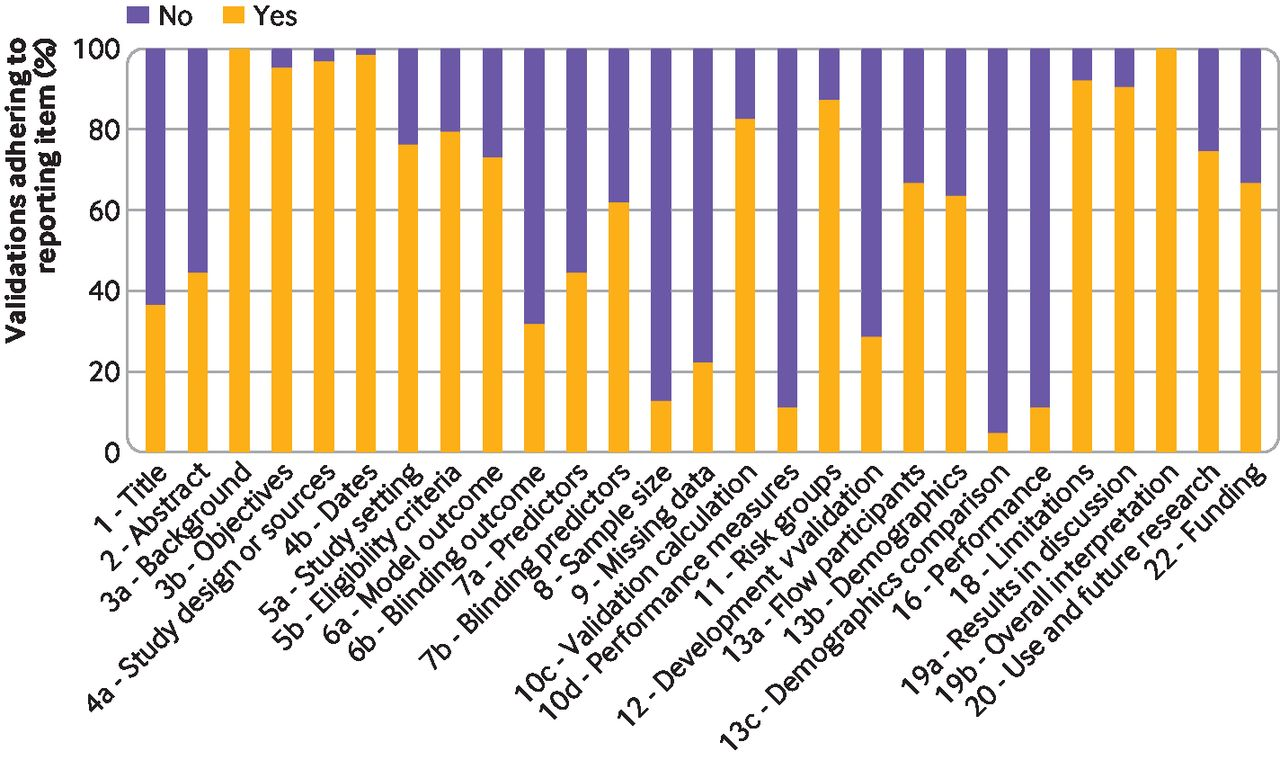
\includegraphics[width=0.8\textwidth]{figures/ADNEXSR/F2.large.jpg}
\caption[Adherence to TRIPOD]{Adherence to reporting the TRIPOD (Transparent Reporting of a multivariable prediction model for Individual Prognosis Or Diagnosis) items in 63 validations.}
\label{fig:1:2}
\end{figure}

\begin{figure}
\centering
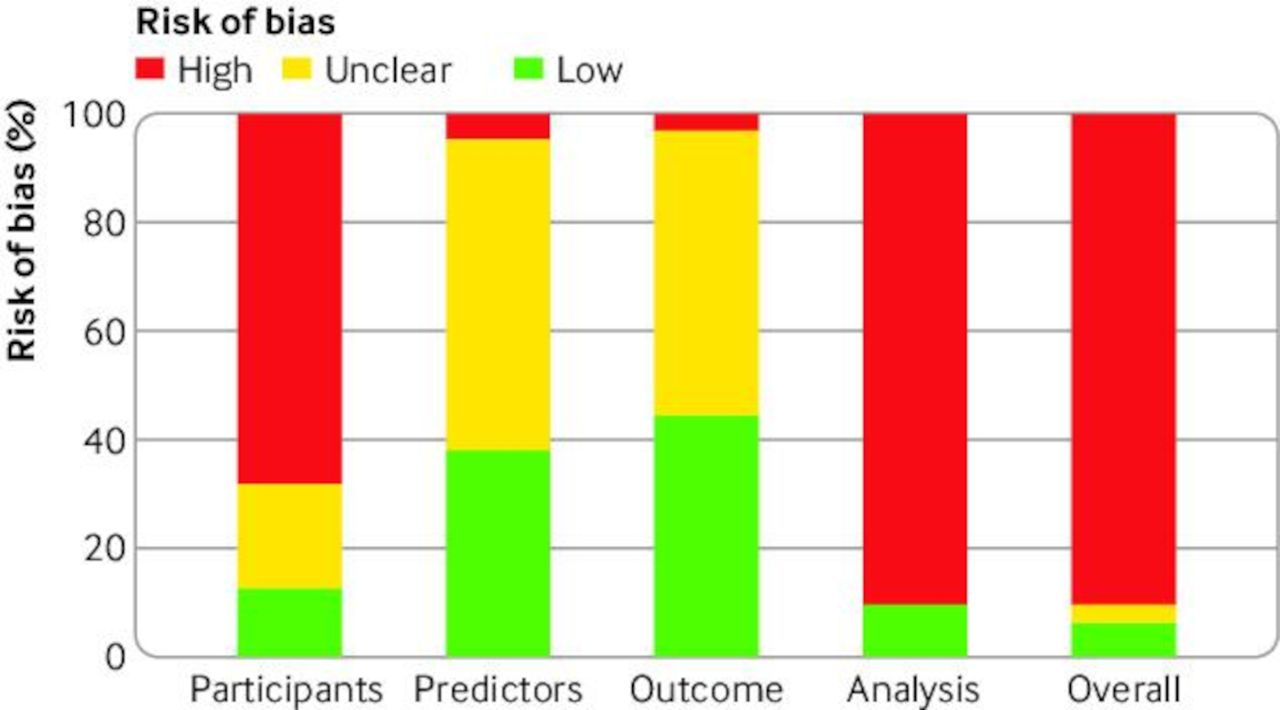
\includegraphics[width=0.8\textwidth]{figures/ADNEXSR/F3.large.jpg}
\caption[Risk of bias overall and by subdomain in 63 validations, assessed by PROBAST]{Risk of bias overall and by subdomain in 63 validations, assessed by PROBAST (Prediction model Risk Of Bias Assessment Tool).}
\label{fig:1:3}
\end{figure}
Fifty-seven (90\%) of 63 validations were rated as having a high risk of bias, two (3\%)
as uncertain risk of bias, and four (6\%) as low risk of bias (Figures \ref{fig:1:3}, S2-5,
\gls{OSF} Extraction sheet) \cite{barrenadaADNEXRiskModel2025}. Forty three (68\%) validations had a high risk of bias for the participant domain, mostly by having incomplete data as an exclusion criterion. Fifty seven (90\%) validations had a high risk of bias for the analysis domain, mostly because of small sample size (69\%; ie, <100 tumours in the smallest group), not including all participants in the analysis (85\%), inappropriate handling of missing data (82\%), and incomplete evaluation of model performance (89\%, in most instances by not reporting an assessment of calibration).

Adherence to TRIPOD items in 36 studies without a focus on selected histologies or clinical subgroups was, on average, 65\% (17.47 of 27 items). In these studies, two had a low risk of bias, one had an unclear risk of bias, and 33 had a high risk of bias.



\subsection{Meta-analysis}
The meta-analysis included studies without post hoc selection based on histology and without a focus on a clinical subgroup only (n=36) that reported the meta-analysed metrics. Only two studies included in the meta-analysis used tumour as the unit of study
 \cite{behnamfarComparisonUltrasoundTumor2022,esquivelvillabonaTwoStepStrategyOptimizing2022}.

The AUC for benign versus malignant tumours in patients who underwent surgery was reported in 12 studies (6309 tumours, 31 centres, and 13 countries) for ADNEX without CA125 (Table
S4 and S6), and the summary AUC was 0.93 (95\% confidence interval 0.91 to 0.94, 95\% prediction interval 0.85 to 0.98) (Table \ref{tab:2}, Figure \ref{fig:1:4})
 \cite{vancalsterValidationModelsDiagnose2020,chenComparisonORADSADNEX2022,
  diazOvarianTumorsRisk2017a,heEstimatingRiskMalignancy2021,
  hiettPerformanceIOTASimple2022,lamhuongOptimalCutOffPoint2022,
  pelayoComparisonUltrasoundScores2023,pengEvaluationDiagnosticValue2021,
  poonyakanokPreoperativeEvaluationADNEX2021,
  qianComparisonDiagnosticPerformances2021,
  sayasnehEvaluatingRiskOvarian2016,
  zhangExternalValidationAssessment2022}.
Twenty one studies (9202 tumours, 43 centres, and 18 countries) reported the AUC for benign versus malignant tumours in patients who underwent surgery for ADNEX with CA125,
 \cite{vancalsterValidationModelsDiagnose2020,araujoPerformanceIOTAADNEX2017,
  behnamfarComparisonUltrasoundTumor2022,chenPerformanceIOTAADNEX2019,
  diazOvarianTumorsRisk2017a,heEstimatingRiskMalignancy2021,
  joyeuxSurgeryPredictabilityMalignant2016,
  lamhuongOptimalCutOffPoint2022,meysEstimatingRiskMalignancy2017,
  namAssessmentDifferentNEoplasias2021,pengEvaluationDiagnosticValue2021,
  poonyakanokPreoperativeEvaluationADNEX2021,
  qianComparisonDiagnosticPerformances2021,
  sayasnehEvaluatingRiskOvarian2016,stukanDevelopmentValidationModel2019,
  szubertPerformanceSelectedModels2020,szubertExternalValidationIOTA2016,
  tugPreoperativeDiscriminatingPerformance2020,vioraADNEXModelTriage2020,
  yangPerformanceIOTAADNEX2022,zhangExternalValidationAssessment2022}
(Table S4 and S6) and the summary \gls{AUC} was 0.93 (\gls{CI} 95\% 0.92-0.94, 95\% \gls{PI}
0.85-0.98) (Table \ref{tab:2}, Figure \ref{fig:1:5}).

\begin{figure}
\flushleft
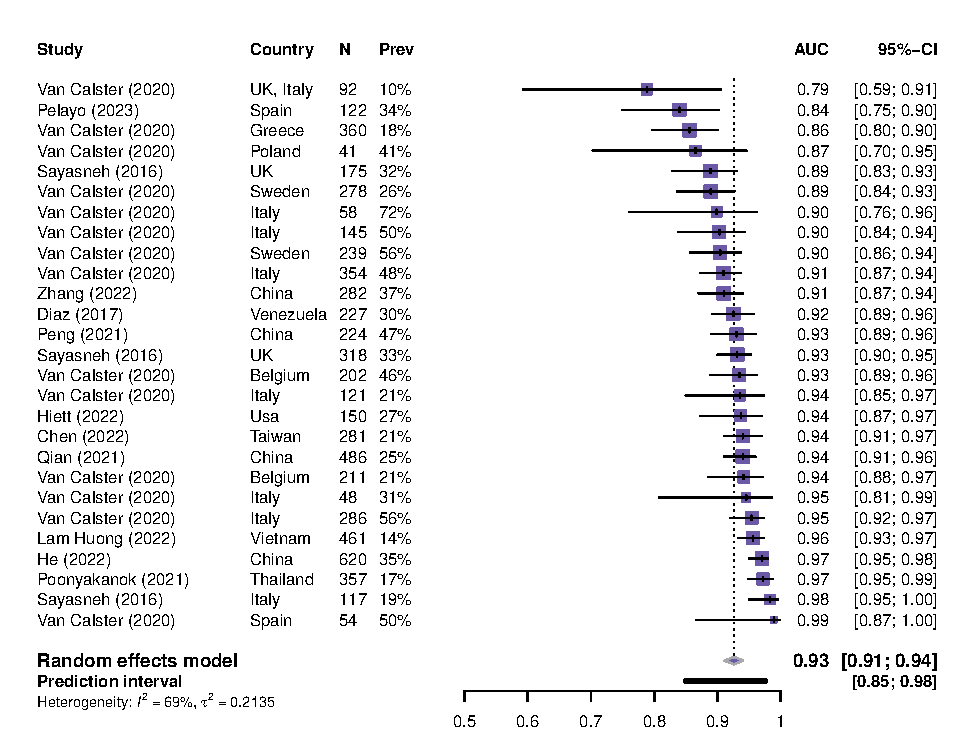
\includegraphics[width=1\textwidth]{figures/ADNEXSR/Figure4.pdf}
\caption[Forest plot AUC ADNEX without CA125]{Forest plot of area under the receiver operating curve in studies where the ADNEX (Assessment of Different Neoplasias in the adnexa) model was used without CA125 (cancer antigen 125). Results in the forest plot are centre specific results, so studies with more than one centre can appear multiple times. CI=confidence interval}
\label{fig:1:4}
\end{figure}

\begin{figure}
\flushleft
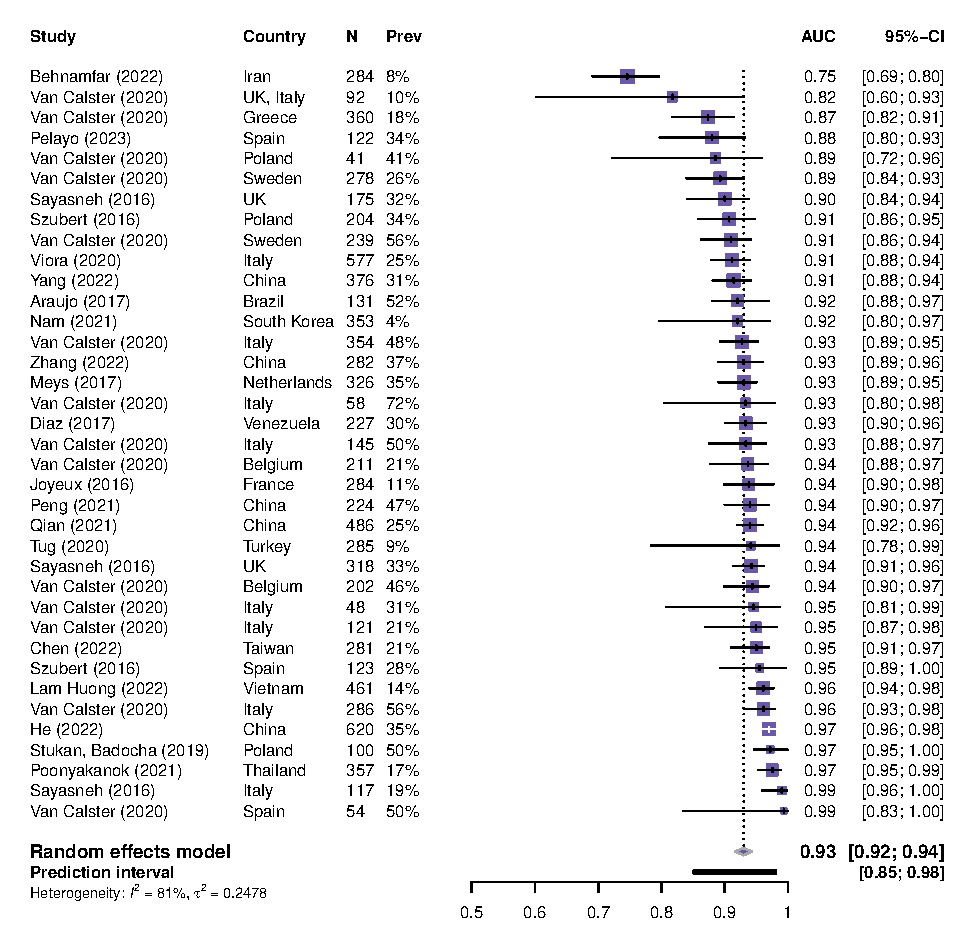
\includegraphics[width=1\textwidth]{figures/ADNEXSR/Figure5.pdf}
\caption[Forest plot AUC ADNEX with CA125]{Forest plot of area under the receiver operating characteristic curve in studies where the ADNEX (Assessment of Different Neoplasias in the adnexa) model was used with CA125 (cancer antigen 125). Results in the forest plot are centre specific results, so studies with more than one centre can appear multiple times. CI=confidence interval}
\label{fig:1:5}
\end{figure}




Sensitivity and specificity at the 10\% risk of malignancy threshold in patients who underwent surgery were reported in 10 studies for ADNEX without CA125 (Tables S4 and S7)
 \cite{vancalsterValidationModelsDiagnose2020,chenComparisonORADSADNEX2022,
  diazOvarianTumorsRisk2017a,hiettPerformanceIOTASimple2022,
  lamhuongOptimalCutOffPoint2022,pelayoComparisonUltrasoundScores2023,
  poonyakanokPreoperativeEvaluationADNEX2021,
  qianComparisonDiagnosticPerformances2021,
  sayasnehEvaluatingRiskOvarian2016,
  zhangExternalValidationAssessment2022}.
The summary sensitivity and specificity were 0.93 (95\% confidence interval 0.90 to 0.95, 95\% prediction interval 0.73 to 0.99) and 0.75 (95\% confidence interval 0.70 to 0.79, 95\% prediction interval 0.46 to 0.91), respectively (Figures \ref{fig:1:6} and S8)
 \cite{vancalsterValidationModelsDiagnose2020,
  jeongValidationIOTAADNEXModel2020,araujoPerformanceIOTAADNEX2017,
  chenComparisonORADSADNEX2022,diazOvarianTumorsRisk2017a,
  heEstimatingRiskMalignancy2021,
  joyeuxSurgeryPredictabilityMalignant2016,laiComparisonORADSGIRADS2022,
  lamhuongOptimalCutOffPoint2022,meysEstimatingRiskMalignancy2017,
  namAssessmentDifferentNEoplasias2021,
  pelayoComparisonUltrasoundScores2023,pengEvaluationDiagnosticValue2021,
  poonyakanokPreoperativeEvaluationADNEX2021,
  qianComparisonDiagnosticPerformances2021,
  sandalComparisionRiskMalignancy2018a,sayasnehEvaluatingRiskOvarian2016,
  stukanDevelopmentValidationModel2019,szubertExternalValidationIOTA2016,
  tugPreoperativeDiscriminatingPerformance2020,vioraADNEXModelTriage2020,
  wangEvaluatingRiskMalignancy2023,yangPerformanceIOTAADNEX2022,
  zhangExternalValidationAssessment2022}.
For ADNEX with CA125, sensitivity and specificity at the 10\% risk of malignancy threshold in patients who underwent surgery were reported in 23 studies (Table S4 and table S7). The summary sensitivity and specificity were 0.94 (95\% confidence interval 0.92 to 0.95, 95\% prediction interval 0.80 to 0.98) and 0.77 (95\% confidence interval 0.73 to 0.81, 95\% prediction interval 0.47 to 0.93), respectively (Figure \ref{fig:1:7} and S8)

Net benefit and relative utility were calculated based on studies that presented sensitivity and specificity at the 10\% risk of malignancy threshold in patients who underwent surgery (Table
S7). For ADNEX without CA125, the summary net benefit was 0.28 (95\% confidence interval 0.21 to 0.35, 95\% prediction interval 0.05 to 0.68) and the summary relative utility was 0.50 (95\% confidence interval 0.37 to 0.62, 95\% prediction interval −0.44 to 0.79). The probability that the model is clinically useful in a random new centre was estimated to be 91\% (Table S9, Figure S6, and Figure S7). For ADNEX with CA125, the summary net benefit was 0.28 (95\% confidence interval 0.22 to 0.33, 95\% prediction interval 0.05 to 0.65), and the summary relative utility was 0.54 (95\% confidence interval 0.45 to 0.61, 95\% prediction interval −0.12 to 0.78). The probability that the model is clinically useful in a random new centre was estimated to be 95\% (Table S9, Figure S8-9).

Pairwise AUC values in patients who underwent surgery were reported in four studies for ADNEX without CA125 and in five studies for ADNEX with CA125 (Table S10)
 \cite{vancalsterValidationModelsDiagnose2020,
  poonyakanokPreoperativeEvaluationADNEX2021,
  sayasnehEvaluatingRiskOvarian2016,vioraADNEXModelTriage2020,
  zhangExternalValidationAssessment2022}.
The summary pairwise AUC values for ADNEX without CA125 ranged from 0.66 (stage II-IV primary invasive v metastatic) to 0.97 (benign v stage II-IV primary invasive) (Table S11). For ADNEX with CA125, the summary pairwise AUC values ranged from 0.72 (borderline v stage I primary invasive) to 0.98 (benign v stage II-IV primary invasive).

\begin{figure}
\flushleft
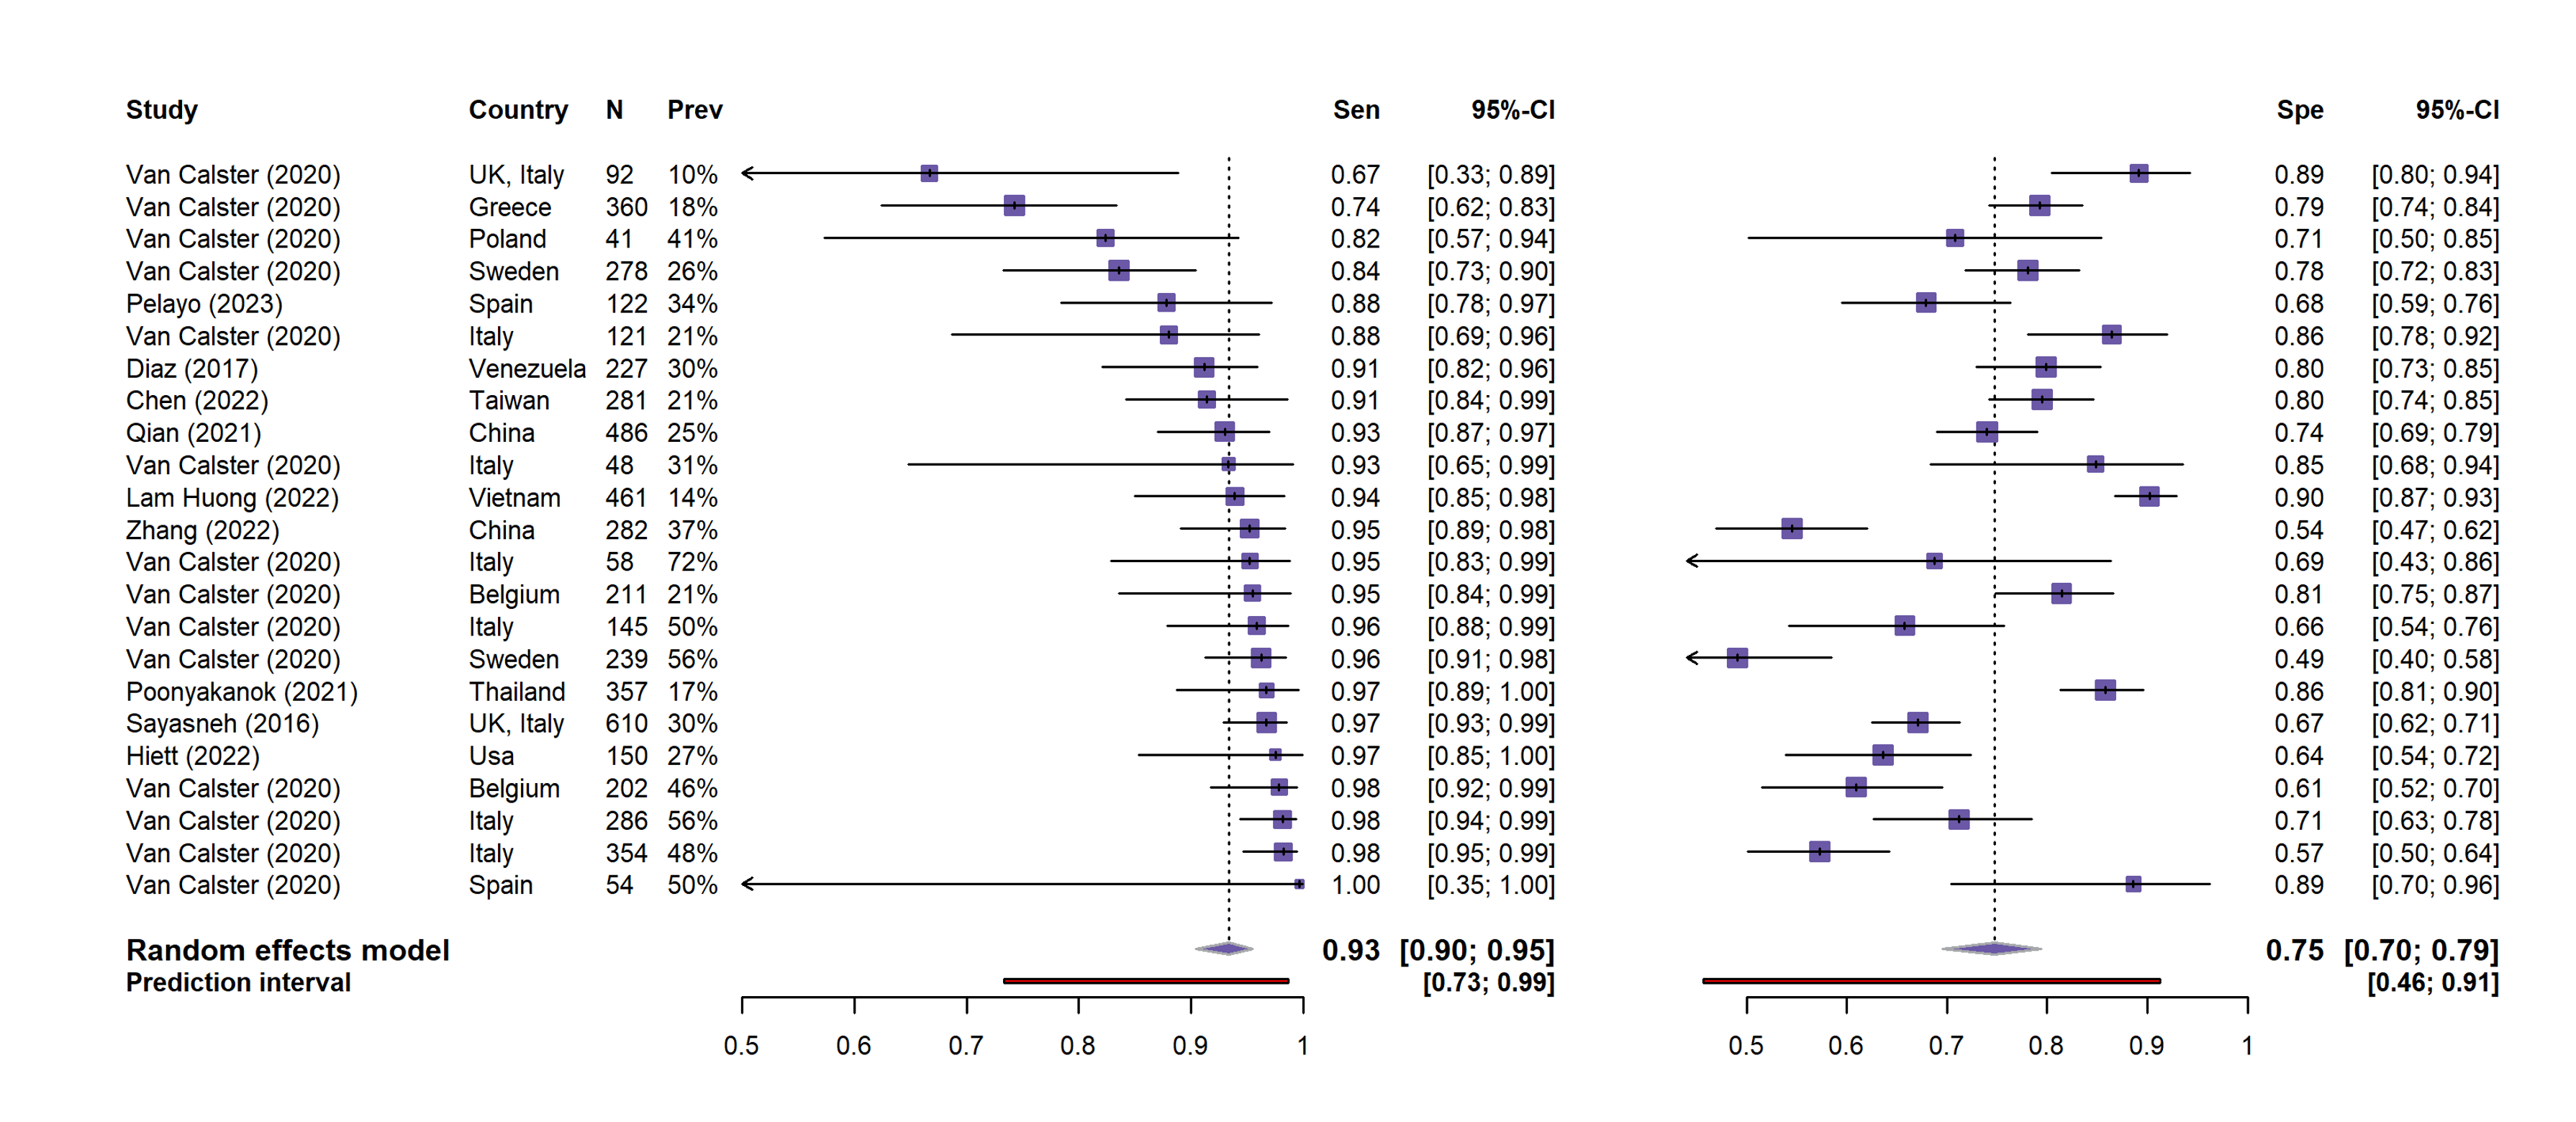
\includegraphics[width=1\textwidth]{figures/ADNEXSR/Figure6.png}
\caption[Forest plot sensitivity and specificity ADNEX without CA125 at 10\% risk of malignancy]{Forest plot of sensitivity and specificity at the 10\% risk of malignancy threshold in studies where the ADNEX (Assessment of Different Neoplasias in the adnexa) model was used without CA125 (cancer antigen 125). Results in the forest plot are centre specific results, so studies with more than one centre can appear multiple times. CI=confidence interval}
\label{fig:1:6}
\end{figure}

The AUC for benign versus malignant tumours in patients managed with and without surgery combined was reported in two studies (5167 tumours, 18 centres, and eight countries) with a summary estimate of 0.94 (95\% confidence interval 0.93 to 0.96, 95\% prediction interval 0.88 to 0.99) for ADNEX with CA125  (Table \ref{tab:2})
 \cite{vancalsterValidationModelsDiagnose2020,hackExternalValidationORADS2022}.
\gls{ADNEX} without CA125 was assessed in only 1 study (4905 tumours, 17 centres, seven
countries) \cite{vancalsterValidationModelsDiagnose2020}. This study reported a summary AUC of 0.94 (95\% confidence interval 0.91 to 0.95, 95\% prediction interval 0.82 to 0.98)..

Table \ref{tab:2} and Tables S6-9 present the sensitivity and subgroup results for AUC, specificity, sensitivity, net benefit, and relative utility. These results showed that the findings were robust (AUC values ranged from 0.90 to 0.95 across all analyses) and clinical utility was suggested in all subgroups. When limiting the analyses to studies with a low risk of bias, summary AUC values were 0.93 (with CA125) and 0.91 (without CA125). Sensitivity was higher and specificity lower in oncology versus non-oncology centres and in patients who were postmenopausal versus premenopausal. In line with these findings, meta-regression suggested that the prevalence of malignancy was not related to AUC but was related positively to sensitivity and negatively to specificity (Figures S10-12).


\begin{figure}
\flushleft
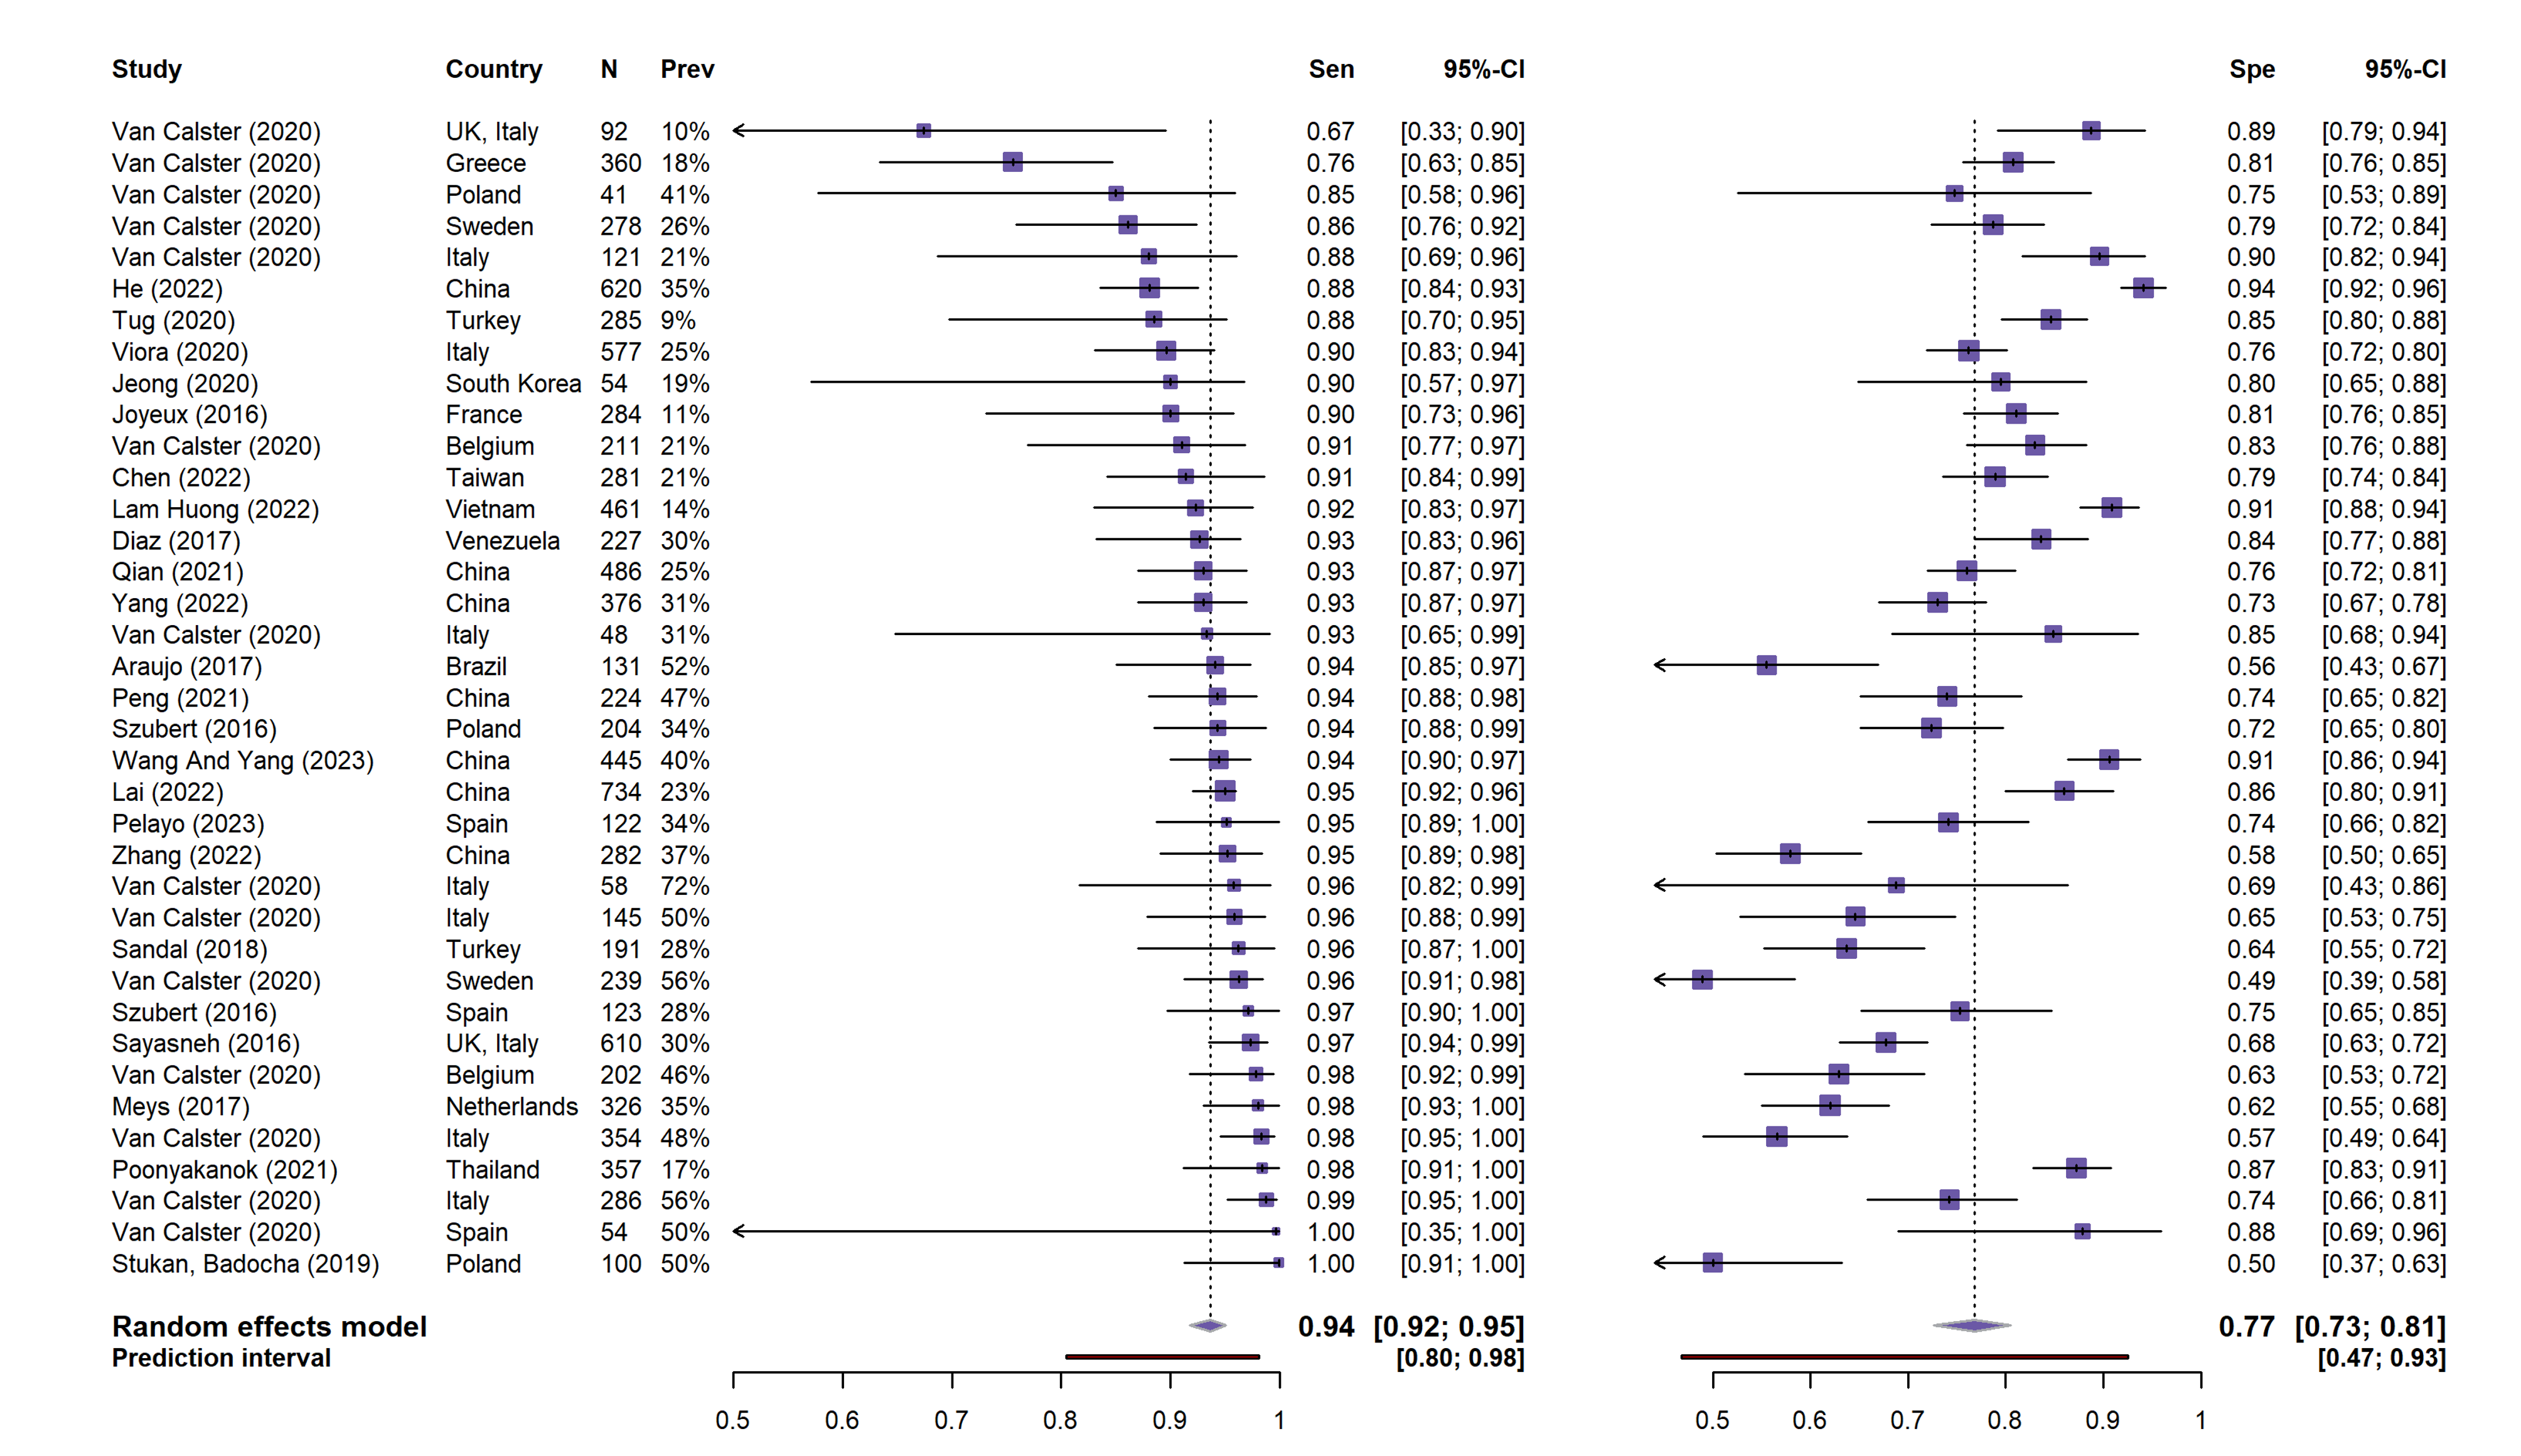
\includegraphics[width=1\textwidth]{figures/ADNEXSR/Figure7.png}
\caption[Forest plot sensitivity and specificity ADNEX with CA125 at 10\% risk of malignancy]{Forest plot of sensitivity and specificity at the 10\% risk of malignancy threshold in studies where the ADNEX (Assessment of Different Neoplasias in the adnexa) model was used with CA125 (cancer antigen 125). Results in the forest plot are centre specific results, so studies with more than one centre can appear multiple times. CI=confidence interval}
\label{fig:1:7}
\end{figure}



Meta-analysis of calibration only in patients who underwent surgery was not feasible because only one study reported calibration slope and intercept \cite{vancalsterValidationModelsDiagnose2020}. Four studies presented a
calibration plot: in three studies
 \cite{sayasnehEvaluatingRiskOvarian2016,vioraADNEXModelTriage2020,zhangExternalValidationAssessment2022}
the estimated risks were close to the observed risks and in one study
 \cite{vancalsterValidationModelsDiagnose2020} the risk of malignancy was
slightly underestimated (Supplementary material S8).

Based on the subdomains of the GRADE assessment, we found that the risk of bias in the studies included in this meta-analysis was a substantial limitation affecting the certainty of our meta-analysis results. Only two studies (representing 5511 tumours or 32\% of the total tumours included in this review) were not classified as having a high risk of bias,
 \cite{vancalsterValidationModelsDiagnose2020,sayasnehEvaluatingRiskOvarian2016}.
but the sensitivity analysis according to risk of bias showed consistent findings (Table \ref{tab:2}, Table S8 and S9). Funnel plots for AUC did not suggest publication bias (Figure S13).

\section{Discussion}

\subsection{Principal findings}

The ADNEX model performed well in classifying tumours and in differentiating between benign and malignant tumours across various settings and populations. Our results indicated that ADNEX was clinically useful at the 10\% risk of malignancy threshold (eg, to help decide whether a patient should be referred for assessment to a gynaecological oncology centre). We found deficiencies in study reporting, and most studies were judged to have a high risk of bias, but our sensitivity analyses indicated that performance was almost identical in studies with a low risk and high risk of bias.

For ADNEX with CA125, the AUC was 0.93 based on all studies, versus 0.93 when based only on studies with a low risk of bias. For ADNEX without CA125, the AUC values were 0.93 (all studies) and 0.91 (low risk of bias only). High risk of bias was mainly caused by small sample size, no assessment of calibration performance, and unjustified use of complete case analysis. Small sample size implies that the estimated AUC value is less precise but it does not systematically affect the AUC, unless publication bias exists. The funnel plots did not suggest publication bias. Absence of calibration does not affect the AUC. Using complete cases, in terms of CA125 or other predictors, might lead to underestimation of AUC because missing values tend to be associated with the examiner's subjective impression that the tumour is benign
 \cite{landolfoBenignDescriptorsADNEX2023}. Complete case analysis would then tend to exclude clearly benign tumours, which would make the sample more homogeneous and reduce the AUC. Our results, however, suggest that the effect of complete case analysis on performance might have been minimal. The effect on calibration could not be assessed. Taken together, we believe that the results of our meta-analysis are reliable.

 \subsection{Strengths and limitations of this study}

Strengths of our systematic review include meta-analysis of ADNEX both as a risk model and as a diagnostic test, and the thorough critical appraisal of risk of bias and reporting quality with recommended checklists \cite{wolffPROBASTToolAssess2019,collinsTransparentReportingMultivariable2015}.
Our study also had limitations. Some of the authors of this study had a conflict of interest because of their involvement in developing ADNEX or in some of the included external validation studies. To deal with this conflict of interest, independent researchers with expertise in study methodology and prediction modelling evaluated the IOTA related studies. A limitation of our findings (but not of our study) is that calibration performance was reported in only four studies and therefore meta-analysis of calibration was not possible.

\subsection{Comparison with other studies}

Previous systematic reviews have conducted meta-analyses of the diagnostic
performance of \gls{ADNEX} with CA125
 \cite{cuiDiagnosticAccuraciesUltrasound2022,
  davenportMenopausalStatusUltrasound2022,
  huangDiagnosticAccuracyADNEX2021,westwoodRiskScoresGuide2018,
  yueValueAssessmentDifferent2022}.
They used the \gls{QUADAS}-2 tool \cite{whitingQUADAS2RevisedTool2011} to assess risk
of bias, and found between 0-64\% of studies had a high risk of bias in
at least one domain. We identified 45 of 47 studies with a high risk of bias with PROBAST, designed for the appraisal of risk prediction models. None of the previous meta-analyses of ADNEX included clinical utility, calibration, or AUC. Our results align with those of other systematic reviews of risk prediction modelling studies in various domains. These studies consistently indicated that reporting in the original studies was poor and that many studies had a high risk of bias  \cite{collinsExternalValidationMultivariable2014,
  wynantsPredictionModelsDiagnosis2020,
  helmrichDoesPoorMethodological2022,
  dhimanReportingPrognosticClinical2021,andaurnavarroRiskBiasStudies2021,
  alloteyExternalValidationPrognostic2022,
  bouwmeesterReportingMethodsClinical2012}.
The results in terms of sensitivity and specificity of ADNEX in our meta-analysis, however, were similar to those in the other meta-analyses of ADNEX performance.

\subsection{Study implications}

ADNEX is intended for use by gynaecologists to help them decide on the most appropriate management of an adnexal mass detected on ultrasound. Our findings support the use of ADNEX in choosing between surgery and conservative follow-up. Conservative follow-up might be appropriate in patients with a low risk of malignancy (eg, <1\%, based on meta-analysis of patients managed with and without surgery). Our results also support the use of ADNEX in deciding on the most appropriate management if conservative management is not suitable (eg, surgery at a local hospital if the risk of malignancy is <10\% or referral to an oncology centre if the risk is>10\%; based on meta-analysis of patients who underwent surgery) \cite{timmermanESGOISUOGIOTA2021}.

ADNEX can also be helpful in deciding on the management of a suspected malignancy (ie, investigations to find the primary tumour if a metastasis in the ovary is likely, or fertility sparing surgery if a borderline tumour is likely; based on meta-analysis in patients who underwent surgery). Because the AUC values of ADNEX with and without CA125 were similar, and because adding CA125 mainly helps to distinguish between different types of malignant tumours, we argue that the main use of ADNEX without CA125 is to help decide whether conservative follow-up, surgery in a local centre, or referral to an oncology centre is appropriate. The main use of ADNEX with CA125 is to help decide on the optimal management of a tumour suspected to be malignant, because it differentiates better between malignant subtypes than ADNEX without CA125.

Although our findings suggest that ADNEX is clinically useful, well conducted validations of any model are always of value to monitor its performance in diverse regions and clinical settings, and over time \cite{vancalsterThereNoSuch2023}. To improve the performance of ADNEX even more, efforts to update the ADNEX formula are of interest \cite{vancalsterThereNoSuch2023,
  onbehalfoftopicgroupevaluatingdiagnostictestsandpredictionmodelsofthestratosinitiativeCalibrationAchillesHeel2019}.
If further validation studies are conducted, we recommend including a validation of ADNEX without CA125, using a sufficiently large sample that allows calibration and multinomial discrimination to be assessed, and including patients irrespective of whether they are managed surgically or non-surgically (despite the challenges about reference standard for patients managed without surgery) \cite{vancalsterAssessingDiscriminativeAbility2012,vanhoordeAssessingCalibrationMultinomial2014}.
Methodological recommendations for validation studies include using available tools to guarantee adequate sample size, describe missing data in detail and use methods such as imputation when needed, and assess calibration performance \cite{steyerbergClinicalPredictionModels2009,
  onbehalfoftopicgroupevaluatingdiagnostictestsandpredictionmodelsofthestratosinitiativeCalibrationAchillesHeel2019,
  pateMinimumSampleSize2023,rileyMinimumSampleSize2021,
  siskImputationMissingIndicators2023}.
Adherence to the TRIPOD reporting checklists is important to maximise the value of the validation study (\url{https://www.tripod-statement.org}).


\section{Conclusion}
ADNEX has been validated in many studies, with AUC values >0.90 in differentiating between benign and malignant tumours in various settings, and with strong results for its clinical utility at the 10\% risk of malignancy threshold. Because of the lack of assessment of calibration in most studies, evaluating the accuracy of the estimated risks in a substantial way was not possible in this study.


\section*{Other information}

\subsection*{Contributors}
Contributions were based on the CRediT taxonomy. LB contributed to conceptualisation, project administration, project administration, methodology, resources, investigation, validation, data curation, software, formal analysis, visualisation, writing of the original draft of the manuscript, and review and editing of the manuscript; AL contributed to resources, investigation, validation, data curation, and review and editing of the manuscript; PD contributed to validation, and review and editing of the manuscript; GC contributed to methodology, validation, and review and editing of the manuscript; LW contributed to methodology, software, formal analysis, and review and editing of the manuscript; JYV contributed to methodology, data curation, and review and editing of the manuscript; DT contributed to funding acquisition, and review and editing of the manuscript; LV contributed to investigation, data curation and review and editing of the manuscript; BVC contributed to conceptualisation, funding acquisition, supervision, methodology, investigation, validation, data curation, software, formal analysis, writing of the original draft of the manuscript, and review and editing of the manuscript. All authors have read, share final responsibility for the decision to submit for publication, and agree to be accountable for all aspects of the work. BVC is the guarantor. The corresponding author attests that all listed authors meet authorship criteria and that no others meeting the criteria have been omitted. Transparency statement: The lead author affirms that this manuscript is an honest, accurate, and transparent account of the study being reported; that no important aspects of the study have been omitted; and that any discrepancies from the study as planned (and, if relevant, registered) have been explained.

\subsection*{Funding}
This research was supported by the Research Foundation Flanders (FWO, grant G097322N) with BVC and DT as supervisors. LW and BVC were supported by Internal Funds KU Leuven (grant C24M/20/064). JYV was supported by the National Institute for Health and Care Research (NIHR) Community Healthcare MedTech and In Vitro Diagnostics Co-operative at Oxford Health NHS Foundation Trust. The views expressed are those of the authors and not necessarily those of the NHS, NIHR, or Department of Health and Social Care. GC is supported by Cancer Research UK (programme grant C49297/A27294). PD is supported by CRUK (project grant PRCPJT-Nov21\100021). The funders had no role in considering the study design or in the collection, analysis, interpretation of data, writing of the report, or decision to submit the article for publication.

\subsection*{Competing interests}
All authors have completed the ICMJE uniform disclosure form at \url{https://www.icmje.org/disclosure-of-interest/} and declare: support from Research Foundation Flanders (FWO), Internal Funds KU Leuven, National Institute for Health and Care Research Community Healthcare MedTech, In Vitro Diagnostics Co-operative at Oxford Health NHS Foundation Trust, Cancer Research UK, and CRUK for the submitted work; BVC, LV, and DT are members of the steering committee of the International Ovarian Tumour Analysis (IOTA) consortium and were involved in the development of the ADNEX model; BVC and DT report consultancy work done by KU Leuven to help implement and test the ADNEX model in ultrasound machines by Samsung Medison, GE Healthcare, Canon Medical Systems Europe, and Shenzhen Mindray Bio-medical Electronics, outside the submitted work; GC is a statistics editor for the BMJ; no financial relationships with any organisations that might have an interest in the submitted work in the previous three years; no other relationships or activities that could appear to have influenced the submitted work.


\subsection*{Data availability statement}
Data are available in a public, open access repository. All data relevant to the study are included in the article or uploaded as supplementary information. Some data were provided by the authors and were not public information; therefore this information was omitted from the public repository.

\section*{Acknowledgments}

We thank Thomas Vandendriessche, Chayenne Van Meel, and Krizia Tuand, the biomedical reference librarians of the KU Leuven Libraries (2Bergen, Learning Centre Désiré Collen, Leuven, Belgium) for their help in conducting the systematic literature search. We gratefully acknowledge the authors of the external validation of ADNEX for providing their valuable data.
